\chapter{Background from Web technologies}
\label{chap:background}

In this thesis, we often operate with such concepts as a webpage, HTML, CSS and JavaScript, web element, DOM, XPath, etc. All these terms refer to the field of web development. In this chapter, we will discuss the meaning of these concepts as well as related works in this area.\\

We will start from the webpage and its main components. Then we will explain in details the algorithm of web page rendering, so called the critical rendering path. After this, we will talk about Web extraction and list the most popular techniques. In the last section, we will discuss related primary works in the field of Web Extraction, especially those which related to the extraction of events and other specific structured information.\\

\section{Web page}
\textit{A Webpage} is primarily text document formatted and annotated with Hypertext Markup Language (HTML). A website is a collection of related webpages together with corresponding media files. To view a rendered webpage, we need to make use of a web browser, which provides communication between the user, webpage resources and web server where the associated website hosted. To get the information needed for a displaying a webpage the browser retrieves the data from a web server by sending HTTP requests. We won't discuss the process of requesting, rather we will explain the intermediate steps between the stage when the browser retrieved the information from the server and displayed it to the user.\\ 

The access to the webpage might be done directly through the HTTP protocol (for example from the terminal) or with the browser which will render the page. In case we do it through the HTTP request, we will get the raw information the same as a browser gets before it does all complicated prepossessing steps and displaying. In the current thesis, we will use both approaches and take advantage of each of them.

There are two main types of the website and therefore the pages - \textit{static} and \textit{dynamic}. A static webpage is usually written in a plain HTML, whereas dynamic page is using server-side scripts for the content generation. The main points which make the differences between them are scalability, simplicity to update the content and the price. With dynamic websites, it is easy to create a significant number of similar pages and dynamically update the content based on user actions. Dynamic pages are taking it's content from a database, whereas the static pages already have some content which can't be updated quickly. But at the same time with a dynamic website, it is more complicated to change the design, because the pages are essentially a template into which content is poured to. The design of static pages is more flexible and can be modified manually. As for the price, static website is relatively cheap and easy to make comparing to dynamic websites.\\ 

Anyways, after the browser retrieved the information from the server, for both dynamic and static webpages the browser has the same types of information to display the webpage. Only in static case the browser retrieved original files (HTML, CSS, JavaScript, etc)  with the predefined content, and in the dynamic case the web server generated these files and took the data from a database.\\

A webpage as a set of available information contains a lot of different pieces:

\begin{itemize}
    \item The textual information which we see
    \item HTML code with the content, hyperlinks, buttons and other components which the user can interact with.
    \item Static media files, i.e. images, icons, video files, animated GIF, SVG, textual documents and other attached files.
    \item Dynamic media as Flash, Java applets.
    \item Semantic meta-information about the content of the page.
    \item JavaScript scripts which add interactivity and additional functionality.
    \item Cascading Style Sheets (CSS) files which define how to rendered the webpage and set such properties as a font size, distances between blocks, colors, etc. There are more than five hundreds different CSS properties there.
\end{itemize}

\subsection{HTML, CSS and JavaScript}
The triad of the most important Web technologies are HTML to specify the content of web pages, CSS to specify the presentation of web pages, and JavaScript to specify the behavior of web pages.\cite{JSBook}[source Flanagan, David. JavaScript - The definitive guide (6 ed.). p. 1.]. Let's briefly discuss how these three major components looks like and show small examples.\\
\cite{W3Schools} [source https://www.w3schools.com]\\

\noindent\textbf{Hypertext Markup Language (HTML)} - is the standard markup language for creating web pages and web applications. HTML document has the structure of a tree and contains the configuration of the page, its textual content and links to all associated media files. HTML file is parsed by a browser into Document Object Model and we will consider this process in details in the next section. The building blocks of an HTML is an HTML tags ( \textt{<div>, <title>, <body>})  which after the parsing transformed to an HTML elements. Here is a \nameref{lst:html}: \\

\begin{lstlisting}[language=html, caption={Small example of HTML file}, label={lst:html}, captionpos=b]
<!DOCTYPE html>
<html>
<title>HTML Tutorial</title>
<body>

<h1>This is a heading</h1>
<div>This is a block of information.</div>

</body>
</html>
\end{lstlisting}

It is possible to incorporate both CSS and JavaScript into the HTML, but in a modern web development, these three things are normally separated into different files. It allows to maintain and change the content, the visualization, and the interactivity features independently.\\

Since the HTML document has a structure and consists of these labeled blocks (sometimes even semantic ones as \textt{<title>}), one can consider a web document as a semi-structured document when compared to a plain text document.\\

\noindent\textbf{Cascading Style Sheets (CSS)} is a style sheet language used for describing the presentation of a document written in a markup language \cite{CSSMoz} [source: "CSS developer guide." Mozilla Developer Network. Retrieved 2015-09-24.]. CSS is primarily designed to enable the separation of content and presentation of a webpage, including layout, colors, and fonts. Such separation improves content accessibility and allows easily change the visual presentation of the page. CSS also allows controlling how the page will be displayed on different screens and devices. There are more than five hundred available CSS properties which can be specified. World Wide Web Consortium (W3C) maintain Both the CSS and HTML specifications. The web browser parses CSS files and creates CSSOM tree which is very conceptually similar to DOM. Here is a \nameref{lst:css}: \\

\begin{lstlisting}[language=css, caption={Small example of CSS file}, label={lst:css}, captionpos=b]
body {
    background-color: lightblue;
}

h1 {
    color: white;
    text-align: center;
}

div {
    font-family: verdana;
    font-size: 20px;
}
\end{lstlisting}\\

\noindent\textbf{JavaScript (JS)} is a powerful multi-paradigm language, supporting object-oriented, imperative, and functional programming styles [link to Wiki]. 95\% of 10 million most popular web pages use JS, and all modern web browsers support it without the need for plug-ins [https://w3techs.com/technologies/details/cp-javascript/all/all]. Scripts are embedded in or included to HTML pages and interact with the DOM and CCSOM. JS can interact and modify both DOM and CCSOM, and it adds interactivity to original static webpages. There is an examples of the JS code in listing \ref{lst:js}:

\begin{itemize}
    \item It allows loading data from the server without needs to reload the page (AJAX technology).
    \item It adds animation, interactivity and media content.
    \item It can track the user behavior on the website and collect the information for the web analytic, ad tracking, and penalization purposes.
\end{itemize}

\begin{lstlisting}[language=JavaScript, caption={Small example of JavaScript code}, label={lst:js}, captionpos=b]
var canvas = document.createElement('canvas');
canvas.width = 100;
canvas.height = 100;

var image = new Image();
image.width = 120;
image.height = 150;
image.onload = window.setInterval(function() {
    rotation();
}, 1000/60);
\end{lstlisting}\\


\section{How does the browser render the page}
\label{sec:browser}

Every time the browser retrieves the information from the web server, it makes the series of important actions to display the initial page to the user. This sequence of steps is named \textit{the critical rendering path}. For web developers, it is critical to understand these actions because optimized websites are easy to use and have a higher rank in search engines. Optimized in this case means that the browser can load and render the page quickly and the internal structure of the code is clear.\\

\cite{GoogleDev}[source: https://developers.google.com/web/fundamentals/performance/critical-rendering-path/adding-interactivity-with-javascript]
[source: https://varvy.com/pagespeed/critical-render-path.html]
The algorithm of how does the browser render the page as follows:

\begin{enumerate}
    \item The browser retrieves the HTML, read it and see that there are CSS and JavaScripts files for this HTML needed.
    \item The browser decides if it's possible to render the page and if yes it loads all necessary resources including CSS, JavaScript and media files.
    \item The browser parses the HTML code and builds the \textit{Document Object Model} (DOM) tree. The DOM contains the objects which define the structure and the content of the page.
    \item The browser parses the CSS files and builds the CSSOM tree. It is very much like DOM for HTML. The CSSOM contains the objects which define the style of all elements in DOM.
    \item JavaScript can modify existing DOM and CSSOM, change any elements of both trees.
    \item The DOM and CSSOM trees are combined to form \textit{the Render tree}. Render tree doesn't include the hidden nodes as a script, meta tags, and so on. Also, some nodes are hidden because it was reflected in the CSS files (explicit property "display: none"). Render tree contains only the nodes which required to render the page.
    \item The browser is building the layout and computes the exact position and size of each object.
    \item The painting stage is when the browser takes the render tree and renders (meaning draws) the pixels to the screen of the user. 
\end{enumerate}

On the picture \nameref{fig:domcsstree} you can see how the DOM, CSSOM amd Render Tree look like on the \nth{6} step.\\

\begin{figure}[h]
\begin{center}
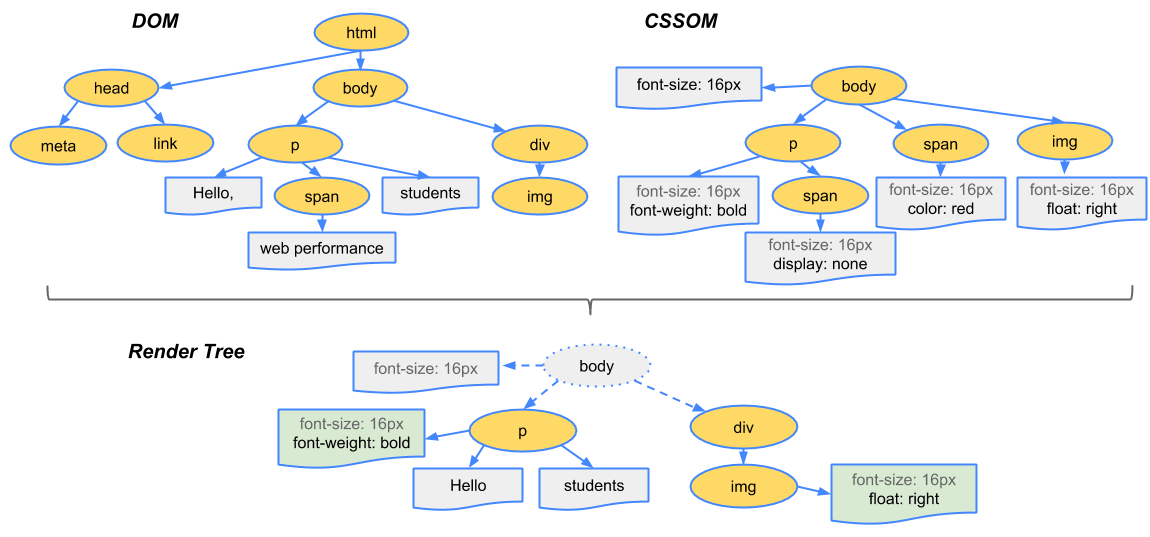
\includegraphics[width=1.0\textwidth]{figures02/render-tree-construction}
\caption{The DOM and CSSOM trees are combined to form the Render tree}
\source{\href{https://developers.google.com/web/fundamentals/performance/critical-rendering-path/render-tree-construction}{https://developers.google.com/}}
\label{fig:domcsstree}
\end{center}
\end{figure}

\subsection{XPath and CSS selectors}
\label{subsec:xpathcss}

\textit{XPath} is a query language for selecting nodes from an XML document based on its tree structure. \textit{CSS selectors} are patterns used to choose the element for styling, and it's also based on a tree structure of an XML document. Since a browser parses and translates an HTML document to a DOM tree, both the XPath and CSS selectors provide the ability to navigate around the tree and select nodes by a variety of criteria. Both CSS and XPath are the languages developed and recommended by World Wide Web Consortium (W3C). Even though we see the similarity between them and they aim to do the same things, XPath and CSS locators have important technical differences:
\begin{itemize}
    \item XPath engines are different in each type of the browser. That means this language is inconsistent and expressions must be rewritten for every browser.  
    \item Some browsers even don't have native support for XPath (Internet Explorer).
    \item XPath has more complex syntax comparing to CSS, which expressions are usually shorter and more clear.
    \item XPath supports boolean functions which evaluate an expression and returns true or false. CSS doesn't support this functionality.
    \item CSS selectors are more flexible and have better performance than XPath in all browsers.
    \item XPath can traverse down, and up the DOM, CSS can traverse only down.
    \item CSS fully supports HTML, for example, 'id' and other unique HTML properties of the element can be used.
\end{itemize}

A community of web developers prefers CSS selectors over XPath due its simplicity and performance. In our work, we will use both CSS and XPath locators since we will need features of both of them: traversing the tree and boolean function as well as specific element locations. You can see the syntax of both languages on the table \nameref{table:xpathcss}.\\

\cite{SelenSpeed} [source about the speed http://elementalselenium.com/tips/34-xpath-vs-css-revisited-2]\\
\cite{XpathCssDiff}[source difference http://www.rapidprogramming.com/questions-answers/difference-between-css-and-xpath-css-vs-xpath-1388]\\

\begin{table}[H]
\begin{center}
{\renewcommand{\arraystretch}{2}

\begin{tabular}{| p{5cm} | p{5cm}| p{4cm} |}
\hline
\thead{Selector}    &    \thead{Xpath (1.0 - 2.0)}    &    \thead{CSS (1-3)}  \\
\hline
Whole web page    &    \texttt{xpath=/html }    &    \texttt{css=html} \\
\hline
Whole web page body    &    \texttt{xpath=/html/body}    &    \texttt{css=body} \\
\hline
All text nodes of web page    &    \texttt{//text()}    &    \texttt{NA}  \\
\hline
Element E by absolute reference    &    \texttt{xpath=/html/body/.../E }    &    \texttt{css=body>...>E}  \\
\hline
Element E by relative reference    &    \texttt{//E}    &    \texttt{css=E} \\
\hline
Second E element anywhere on page    &    \texttt{xpath=(//E)[2]}    &    \texttt{NA} \\
\hline
Element E with attribute A    &    \texttt{//E[@A]}    &    \texttt{css=E[A]}  \\
\hline
Element E with attribute A containing text 'A' exactely    &    \texttt{//E[@A='t']}    &    \texttt{css=E[A='t']} \\
\hline
Element E with attribute A containing text 'A'    &    \texttt{//E[contains(@A,'t')]}    &    \texttt{css=E[A*='t']} \\
\hline
Element E whose attribute A ends with 't'    &    \texttt{//E[substring(@A, string-length(@A) - string-length('t')+1)='t']}    &    \texttt{css=xpath=E[A\$='t']}\\
\hline
\end{tabular}}
\caption{Comparison of XPath and CSS selectors syntax}
\source{\href{https://www.simple-talk.com/dotnet/.net-framework/xpath,-css,-dom-and-selenium-the-rosetta-stone/}{Michael Sorens}}
\label{table:xpathcss}
\end{center}
\end{table}


\section{Semantic Web}
Currently, the Internet, in general, can be considered as \textit{"Web of documents"}, where every document is an HTML page. With Semantic Web, W3C is helping to build a technology stack to support a \textit{"Web of data"}, where all available data on those HTML pages produce the database and anyone can retrieve that data similarly working with databases. So \textit{the Semantic Web} is an extension of the Web through the list of specific standards and technologies supported by the W3C \cite{WikiSeman} [source Wiki].  \\

As we know, today not only the humans read the pages on the Internet. A lot of computers with the comprehensive programs read the Interned too, and the easiest example is a search engine. It continuously scans the Web pages, processed an enormous amount of data with complicated algorithms to understand the meaning of the text written in natural language. It is a very complex task to understand the context of the document, its semantic nature and the relationship between included concepts. To do so one needs special software and significant computational power, that's why only big corporations as Google, IBM (with the Watson project), and other can afford it. The root of this complexity lies in the fact that the Web is semi-structured text written in natural language, initially made for simple human needs, not for a computer or complicated queries about the underlying concepts.\\ 

The Semantic Web acts as an integrator of different content and systems. The stack of major technologies as follows: 

\begin{enumerate}
    \item Resource Description Framework (RDF). It is a language for expressing data models, which refer to objects and their relationships. 
    \itme RDF Schema (RDFS), is a vocabulary for describing properties and classes of RDF-based resources.
    \item SPARQ - is a query language for semantic web data sources.
    \item Web Ontology Language (OWL), a family of knowledge. representation. It adds more vocabulary and relations for describing properties and classes.
    \item XML provides basic syntax for the structure of content.
\end{enumerate}

The biggest problem with Semantic Web is its practical feasibility. While learning of HTML is relatively easy, the theoretical background needed to implement the ideas from Semantic web requires the understanding of knowledge representation subject which is quite complicated. 

\subsection{Semantic markup}
\textit{Semantic markup (or semantic annotation)} is an extension of HTML which implies using special tags with meta information. It helps search engines, web crawlers, and browsers automatically retrieve the concepts with detailed information from an HTML page. Search engine relies on this markup to improve search results. For example, it can automatically show the details of a person or a movie right below the search query in case this information appears with the corresponding meta tags on a reliable webpage.\\ 

The list of concepts and its relationships is very broad and includes for example person, address, dates, events, etc. There are three the most popular semantic markup: Microdata, RDF, and Microformat. Also, the last version of HTML (HTML5) has embedded tags which created especially for some semantic annotations. The core of the thesis is using \textit{Microdata} for collecting the initial training set. Let's discuss how does this markup look like and what functionality provide.\\

\subsubsection*{Microdata}
\label{subsubsec:microdata}
\textit{Microdata} vocabularies itself does not provide the semantics or meaning of an Item. \cite{Microdata} [source: https://html.spec.whatwg.org/multipage/microdata.html] Instead of this, web developers can create a custom vocabulary or use vocabularies available on the Web. \textit{Schema.org} schemes provide the most commonly used markup vocabularies, which includes: Person, Place, Event, Organization, and many others. \\

In our work, we regularly use \textit{Event Shcema} vocabulary of the Microdata markup. Let's consider a small example and its primary fields. Look at the two listings: {lst:htmlevent} and {lst:htmleventmark}.\\

\begin{lstlisting}[language=html, caption={Event information without semantic markup}, label={lst:htmlevent}, captionpos=b]
<div class="event-wrapper">
  <div class="event-date">Sat Sep 14</div>
  <div class="event-title">Typhoon with Radiation City</div>
  <div class="event-venue">
    The Hi-Dive
    <div class="address">
        7 S. Broadway<br>
        Denver, CO 80209
    </div>
  </div>
  <div class="event-time">9:30 PM</div>
</div>

\end{lstlisting}
\\

\begin{lstlisting}[language=html, caption={Event information annotated with Microdata}, label={lst:htmleventmark}, captionpos=b]
<div class="event-wrapper" itemscope itemtype="http://schema.org/Event">
  <div class="event-date" itemprop="startDate" content="2013-09-14T21:30">Sat Sep 14</div>
  <div class="event-title" itemprop="name">Typhoon with Radiation City</div>
  <div class="event-venue" itemprop="location" itemscope itemtype="http://schema.org/Place">
    <span itemprop="name">The Hi-Dive</span>
    <div class="address" itemprop="address" itemscope itemtype="http://schema.org/PostalAddress">
      <span itemprop="streetAddress">7 S. Broadway</span><br>
      <span itemprop="addressLocality">Denver</span>,
      <span itemprop="addressRegion">CO</span>
      <span itemprop="postalCode">80209</span>
    </div>
  </div>
  <div class="event-time">9:30 PM</div>
</div>

\end{lstlisting}\\


As you can see, the second code block looks more cumbersome because it has a lot of additional annotations. 

\begin{itemize}
    \item \textbf{itemscope} – creates the Item and indicates that descendants of this element contain information about it.\cite{Microdata} [source: https://html.spec.whatwg.org/multipage/microdata.html]
    \item \textbf{itemtype} – a valid URL of a vocabulary that describes the item. In our case it is "http://schema.org/Event" and if you go by thins link, you will find all possible fields and information. 
    \item \textbf{itemprop} - contatining tag holds specific property of the item, for example "location", "startDate", "name".
\end{itemize}

There are dozens of Event properties in "http://schema.org/Event", but in the thesis we consider only four main properties "name", "startDate", "description" and "location". We will call them \textit{event components}.\\

You can mention, that the item can contain a property as well as another item. For example, property "address" includes the item type "http://schema.org/PostalAddress." In the thesis, it would be an additional difficulty during the parsing process because we will need to invoke not only the property but also the properties of all included items to collect the event components. We will discuss it in chapter \nameref{chap:datacollect}. 

\subsubsection*{Semantic markup popularity}

Search engines take advantage of the semantic markup to automatically extract the information, incorporate it into its vertical services and provide a richer browsing experience for users. Despite the fact that search engines encourage and promote the websites which use such markup, in fact, not all of them use it. By statistics only 16\% of the domains use semantic markup, the rest 84\% use standard HTML. That's also the reason why the task of structural information extraction from unstructured web pages is still relevant - most of the data on the Internet is still stored as a plain HTML.\\ 

We can collect popularity of semantic annotations from Web Data Commons web service. In the fourth quarter of 2016, it crawled 34 million pay-level-domains and detected that there are 5.63 million (16.5\%) domains use RDFa, Microdata or Microformat semantic markup on their pages. See the graph \nameref{fig:markup} to explore the numbers. As you can see, Microdata is leading, that's the main reason why we considered to use this annotation in the thesis. \\

\begin{figure}[h]
\begin{subfigure}{.5\textwidth}
  \centering
  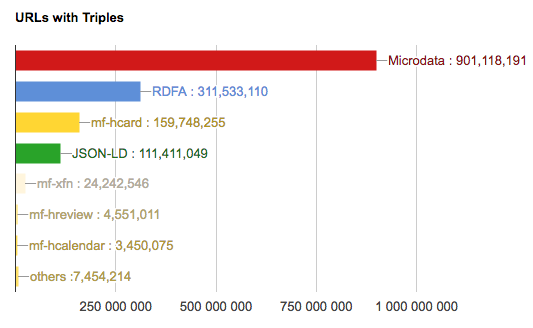
\includegraphics[width=1.\linewidth]{figures02/urls_meta}
  \caption{Across URLs}
\end{subfigure} 
\begin{subfigure}{.5\textwidth}
  \centering
  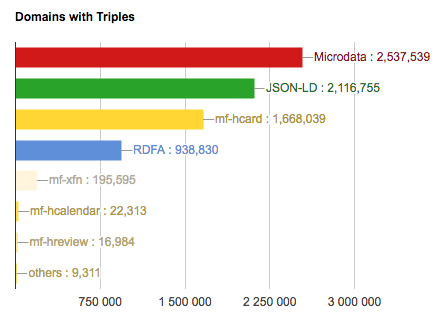
\includegraphics[width=.8\linewidth]{figures02/domain_meta}
  \caption{Across domains}
\end{subfigure}
\caption{Popularity of semantic annotations, 2017}
\source{\href{http://webdatacommons.org/structureddata/2016-10/stats/stats.html}{Web Data Commons}}
\label{fig:markup}
\end{figure}


\section*{Conclusion of the chapter}
In this chapter, we considered the most important concepts which we use in the thesis. We explained the structure of a webpage, discussed related terms like HTML, CSS, and JavaScript, discussed in detail how does the browser render a webpage and the notions of CSS and XPath locators of the web element. Also, we talked about the idea of Semantic Web, its prevalence and described Microdata semantic annotation which we use for collecting the training dataset.\\

In the next chapter, we will cover the Web extraction and theoretical background we apply in the thesis. 